\chapter{Introduction}

\section{Blades Motion}

\begin{figure}[h!]
  \centering
  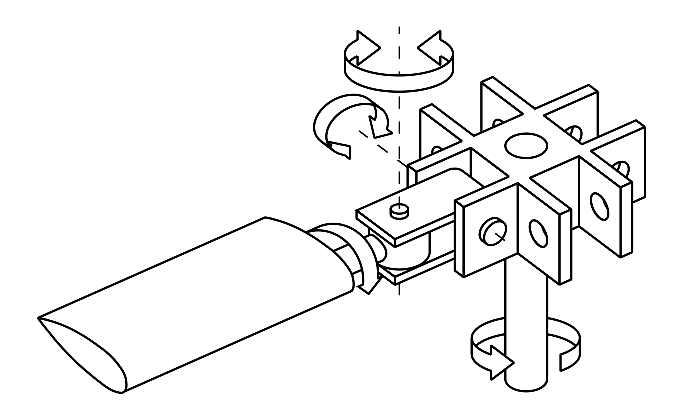
\includegraphics[width=110mm]{eps/rotor_hub_hinges.eps}
  \caption{Rotor blade hinges}
\end{figure}

Neglecting blade flapping motions occuring more frequent than once per revolution flapping angle can be expressed as:

\begin{equation}
\beta \left( \Psi \right)
=
\beta_0 + \beta_{1c} \cos \Psi + \beta_{1s} \sin \Psi 
\end{equation}

\begin{figure}[h!]
  \centering
  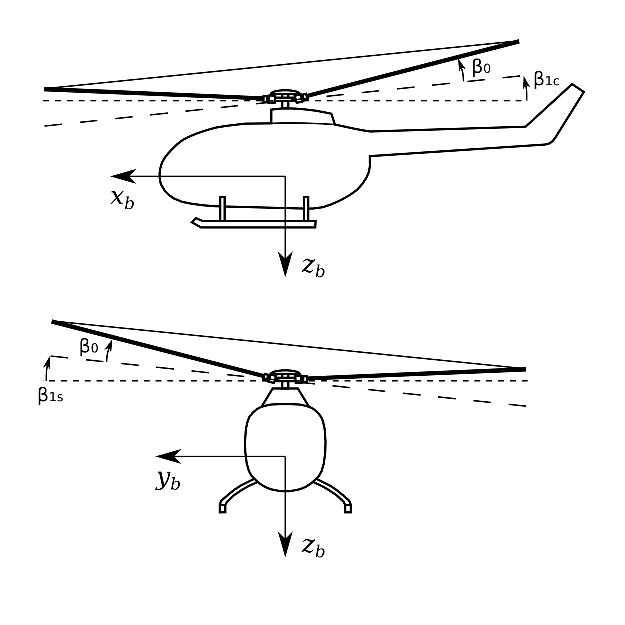
\includegraphics[width=100mm]{eps/rotor_flapping_angles.eps}
  \caption{Rotor disc three degrees of freedom}
\end{figure}

\section{Coordinate Systems Used for Rotor Calculations}

\subsection{Rotor Axis System}

Origin of the Rotor Axis System is coincident with the rotor hub center, the x-axis is positive in forward direction, the y-axis is positive right and z-axis is positive downward direction and it is coincident with the rotor shaft axis.

\begin{figure}[h!]
  \centering
  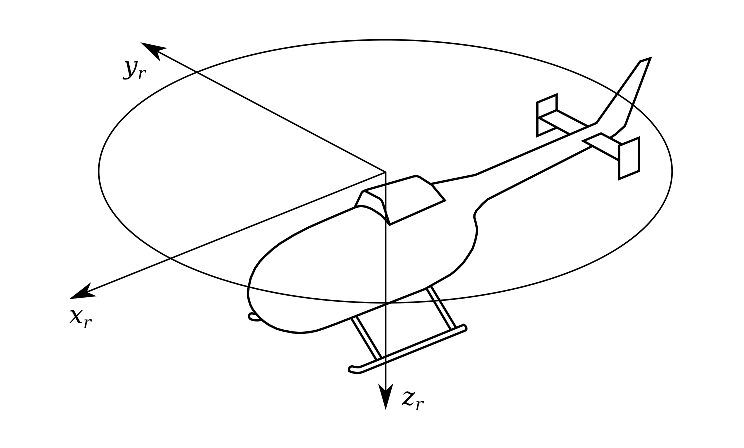
\includegraphics[width=110mm]{eps/coordinate_system_RAS.eps}
  \caption{Rotor Axis System}
\end{figure}

\subsection{Rotor-Wind Axis System}

Rotor-Wind Axis System is very much like Rotor Axis System, the only difference is that it is rotated about z-axis in such a manner that x-axis points directly into relative wind, so there is no lateral airspeed component.

\subsection{Control Axis System}

For most purposes, using the Rotor Axis System causes unnecessary complications. It is convenient to use no cyclic feathering axes system. \cite{GessowMyers1985} Origin of the Control Axis System is coincident with the origin of the Rotor Axis System, but it is rotated by angles of the swashplate roll and pitch so there is no cyclic feathering in this coordinate system.

\begin{figure}[h!]
  \centering
  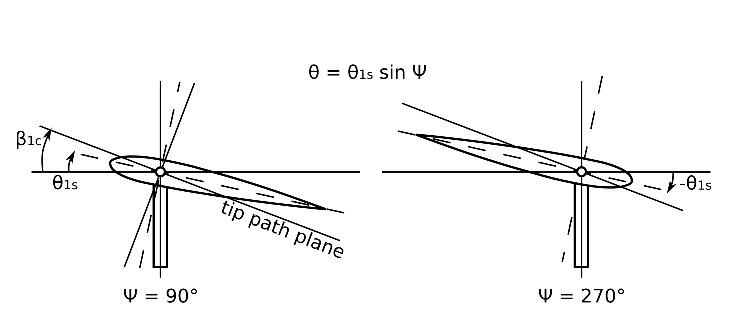
\includegraphics[width=120mm]{eps/rotor_planes.eps}
  \caption{Rotor reference planes}
\end{figure}

\subsection{Disc Axis System}

Origin of the Disc Axis System is coincident with the origin of the Rotor Axis System, but it is rotated by angles of the rotor cone roll and pitch in such a manner that z-axis is perpendicular to the tip path plane so there is no cyclic flapping in this coordinate system.

\subsection{Control-Wind Axis System}

Control-Wind Axis System is very much like Control Axis System, the only difference is that it is rotated about z-axis in such a manner that x-axis points directly into relative wind, so there is no lateral airspeed component.

\subsection{Azimuth Axis System}

Each rotor blade has its own Azimuth Axis System. Origin of the Azimuth Axes System is coincident with the rotor hub center and rotates together with the rotor. The x-axis lies on XY plane of the Rotor Axis System and it is positive toward blade trailing edge, the y-axis lies on XY plane of the Rotor Axis System and points outwards, the z-axis it is coincident with the rotor shaft axis and it is positive in upward direction.

\subsection{Blade Axis System}

Each rotor blade has its own Blade Axis System. Origin of the Blade Axis System is coincident with the point of intersection of flapping and feathering hinge axes. The x-axis lies on XY plane of the Rotor Axis System and it is positive toward blade's trailing edge, y-axis is coincident with the feathering hinge axis and it is positive in outward direction, the z-axis is positive in upward direction.

\begin{figure}
  \centering
  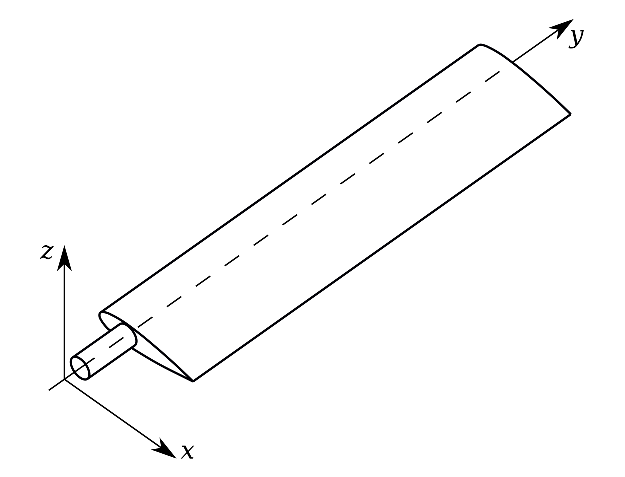
\includegraphics[width=100mm]{eps/coordinate_system_BAS_R.eps}
  \caption{Blade Axis System (right-handed)}
\end{figure}

\begin{figure}
  \centering
  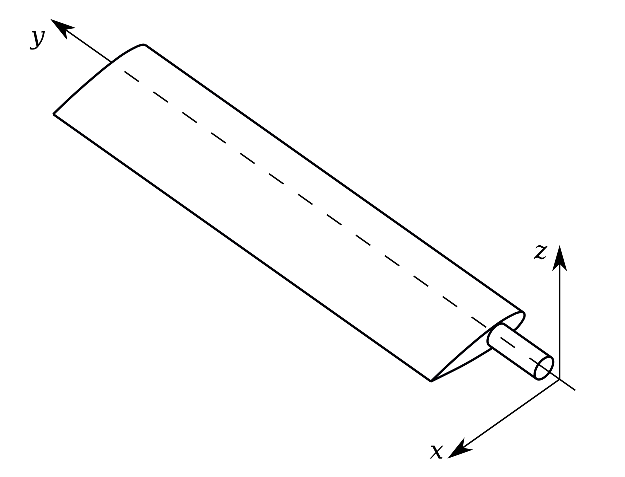
\includegraphics[width=100mm]{eps/coordinate_system_BAS_L.eps}
  \caption{Blade Axis System (left-handed)}
\end{figure}
